As the previous section focused solely on the geometry of the microstructure, we now provide a more comprehensive view of the timescale that drives the interaction between nearest pairs, as well as the times scale involved for the tensor $\textbf{R}(\textbf{x},t)$.

\subsubsection*{A transport equation for the microstructure geometry}
We have seen in the previous section that the tensor $\textbf{R}(\textbf{x},t)$ is able to describe the geometry of the microstructure. 
To determine how this microstructure evolves in time we make use of the transport equation of $P_\text{nst}(\textbf{x},\textbf{r},t,a)$ derived in \citet{zhang2023evolution}.
As it is a rather new formalism we recall this equation here, 
\begin{equation}
    \pddt P_\text{nst}
    + \pdda P_\text{nst}
    + \pddx \cdot  (\textbf{u}^\text{nst}_p P_\text{nst})
    + \pddr \cdot  (\textbf{w}^\text{nst}_p P_\text{nst})
    = \delta(a)P(\textbf{x},\textbf{r},0,t)
    - \frac{P_\text{nst}}{\tau^\text{nst}(\textbf{x},\textbf{r},t,a)}
    \label{eq:dt_Pnst}
\end{equation}
where $\textbf{u}^\text{nst}_p$ and $\textbf{w}_{p}^\text{nst}$ are the conditioned average of the particle phase velocity and relative velocity, respectively, defined \ref{sec:methodo}. 
The left-hand side of \ref{eq:dt_Pnst} corresponds to the convective derivative of $P_\text{nst}$ with respect to the nearest particle statistics' phase space. 
The first term on the right-hand side of \ref{eq:dt_Pnst} account for the creation of the nearest pairs, thus it is non-zero only for the age $a = 0$, as witnessed by the Dirac delta function $\delta(a)$. 
The second term on the right-hand side is the contribution from the destruction of the nearest pairs.
Where we defined $1/\tau^\text{nst}(\textbf{x},\textbf{r},t,a)$ as the rate of destruction of pairs of particles of age $a$ with relative position $\textbf{r}$.
Additionally, we define the mean rate of destruction, $1/\tau_p$, by, 
\begin{equation*}
    \frac{n_p}{\tau_p}(\textbf{x},t) = 
    \int_{0}^\infty
    \int_{\mathbb{R}^3}
    \frac{P_\text{nst} }{\tau^\text{nst}}(\textbf{x},\textbf{r},t,a)
    da d\textbf{r}. 
\end{equation*}
As we show now, $\tau_p$ is of great importance as it governs the timescale of the microstructure.

By taking the partial time derivative of \ref{eq:R}, and utilizing \ref{eq:dt_Pnst}, we obtain an equation for $\textbf{R}(\textbf{x},t)$, it reads,
\begin{equation*}
    \pddt (n_p\textbf{R})
    + \pddx \cdot [n_p(\textbf{u}_p\textbf{R}
    + \textbf{R}^\text{Re})]
    = 
    - \frac{n_p\textbf{R}}{\tau_p}
    +n_p\textbf{B}
    + n_p\textbf{D}
    + n_p\textbf{W}
    \label{eq:dt_R}
\end{equation*}
With,
\begin{align*}
    n_p \textbf{R}^\text{Re}(\textbf{x},t)
    =
    \int_{0}^\infty
    \int_{\mathbb{R}^3}
    \textbf{rr}(\textbf{u}^\text{nst}_p - \textbf{u}_p)
    P(\textbf{x},\textbf{r},t,a)
    d\textbf{r}da,\\
    n_p \textbf{B}(\textbf{x},t)
    =
    \int_{0}^\infty
    \int_{\mathbb{R}^3}
    \textbf{rr}
    P(\textbf{x},\textbf{r},t,0)\delta(a)
    d\textbf{r}da, \\
    n_p\textbf{D}(\textbf{x},t) = 
    \int_{0}^\infty
    \int_{\mathbb{R}^3} \textbf{rr}
    \left[
        \frac{1}{\tau_p(\textbf{x},t)}
        - \frac{1}{\tau^\text{nst}(\textbf{x},\textbf{r},t,a)}
    \right]
    P_\text{nst}
    d\textbf{r}
    da,\\
    n_p \textbf{W}(\textbf{x},t) = 
    \int_{0}^\infty
    \int_{\mathbb{R}^3} \left[
        \textbf{r} \textbf{w}^\text{nst}_p
        + \textbf{w}^\text{nst}_p\textbf{r}
    \right]P_\text{nst}
    d\textbf{r}
    da.
\end{align*} 
The tensor $\textbf{R}^\text{Re}$ represent the flux due to velocity fluctuations. 
The source term $\textbf{B}$ is the averaged square relative position conditioned on the age $a=0$, meaning that it is related to the birth of the nearest particle pairs. 
In opposition to \textbf{D} which is related to the death of the particles pairs due to the presence of $\tau_p$ and $\tau_p^\text{nst}$.
Therefore, $\textbf{D}$ is the weighted average of $\textbf{rr}$ in terms of the destruction rate fluctuation fields. 
Likewise, $\textbf{B}$ is the weighted average of $\textbf{rr}$ on the Dirac distribution $\delta(a)$. 
The former term cancel out under the hypothesis that $1 / \tau^\text{nst}_p(\textbf{x},\textbf{r},t,a)$ is independent of age and relative position, in which case $\tau_p = \tau^\text{nst}_p$. 
Such simplification might be valid at high particle velocities fluctuation, however in our case we could not observe this independence with the DNS results.  
Additionally, the tenor $\textbf{W}(\textbf{x},t)$ is the correlation between the particles relative position and velocity.
Furthermore, due to the presence of the first term on the right-hand side of \ref{eq:dt_R}, we can state that $\textbf{R}(\textbf{x},t)$ will eventually relax within time, and that the relaxation time is $\tau_p$. 
In \citet{zhang2023evolution} they demonstrate that it is also the case for the particle-fluid-particle stress tensor.
In fact, this hold true for all nearest-neighbor averaged particles quantities, since this relaxation time is related to the transport equation of $P_\text{nst}(\textbf{x},\textbf{r},t,a)$, see \ref{eq:dt_Pnst}.
The main takeaway from \ref{eq:dt_R} is that, the microstructure as it is described by $\textbf{R}(\textbf{x},t)$, is motivated by 3 source terms, a term related to the weighted average of $\textbf{rr}$ on pair's birth and on pair's destruction, and a last one related to the particle relative velocity-position correlation. 


Since, $\textbf{R}(\textbf{x},t)$ follow a kinetic theory-like transport equation, it is interesting to discuss the possibility of implementing an equation such as \ref{eq:dt_R} in an Euler-Euler simulation framework. 
Attempting to close the source terms on the right-hand side of \ref{eq:dt_R} is very challenging. 
Instead, one could directly close $\textbf{R}(\textbf{x},t)$ based on the results of \ref{fig:A}, which are statistically steady state results of the microstructure. 
But then, how to know if the inertial effects related to the formation of the microstructure  (left hand-side of \ref{eq:dt_R}) are negligible ?
In fact, provided a relaxation time of the microstructure sufficiently small compared to the timescale of the flow, the derivatives in the right-hand side of \ref{eq:dt_R} might be negligible.
Therefore, $\textbf{R}(\textbf{x},t)$ can be expressed directly in terms of the flow parameters, provided that $\tau_p$ is smaller than the flow timescale. 
Then, the knowledge of $\textbf{R}(\textbf{x},t)$ by either solving \ref{eq:dt_R} or by obtaining direct closures laws, provides useful information for the closure terms in the Euler-Euler model.
For example, the averaged interphase momentum transfer is microstructure dependent. 
This, of course, requires having an expression for the closure terms in terms of the pair distribution function, which is not currently feasible.
Anyhow, the time $\tau_p$ is of major importance for two reasons: 
(1) it determines the timescale at which a statistically steady microstructure might be reached; 
(2) it provides useful information for the modeling of \ref{eq:dt_R}.

\subsubsection*{Mean age of interaction}

In this paragraph we evaluate the mean rate of destruction $1/\tau_p(\textbf{x},t)$. 
It is shown in a few paragraphs that the age distribution function is closely related to the mean rate of destruction. 
Therefore, let's first examine the age distribution, defined as, 
\begin{equation*}
    P_a(\textbf{x},t,a)
    = \frac{1}{n_p(\textbf{x},t)}
    \int_{\mathbb{R}^3}
    P_\text{nst}(\textbf{x},\textbf{r},t,a)
    d\textbf{r}.
\end{equation*} 
It is possible to derive an analytical formula for the age distribution, $P_a(\textbf{x},t,a)$, under the \textit{random destruction assumption} \citep{zhang2023evolution}.
This assumption state that the probability of particle pairs destruction, integrated on all position, is uncorrelated with the age of interaction.
In other worlds, we consider that any pairs of nearest neighbor can be broken apart equally likely regardless of the current age of the particle pair. 
Let us define $1/\tau_p^a(\textbf{x},t,a) = \frac{1}{n_p}\int_{\mathbb{R}^3}\tau^\text{nst} P_\text{nst}d\textbf{r}$, as the mean rate of pair destruction at age $a$, then this hypothesis state that $\tau^a_p$ is not a function of the age, such that $\tau^a_p(\textbf{x},t,a) = \tau_p(\textbf{x},t)$. 
It must be understood that $\tau^a_p$ is independent of the age, which does not imply that $\tau^\text{nst}_p$ is independent of the relative position, $\textbf{r}$, which is not true.
Under this assumption, which will be shown to be valid in our parameters' range, we can derive an analytical formula for the age distribution \citep{zhang2023evolution}, namely,
\begin{align}
    P_a(\textbf{x},t, a)  
    =\frac{e^{-a/\tau_p(\textbf{x},t)}}{\tau_p(\textbf{x},t)}.
    \label{eq:Pa}
\end{align} 
We can see that the age distribution is solely function of $\tau_p(\textbf{x},t)$ and that it is normalized to $1$.
Additionally, with this definition $\tau_p(\textbf{x},t)$, turns out to be equivalent to the first moment of the age distribution, such that, 
\begin{equation*}
    \int_{0}^\infty
    a P_\text{a}(\textbf{x},t,a)
    da
    =\tau_p(\textbf{x},t). 
\end{equation*}
Therefore, $\textbf{R}(\textbf{x},t)$ has a relaxation time equal to the first moment of the age distribution, which can be understood as the mean time of interaction of the particles pairs. 
In this sense it is intuitive to understand that the microstructure reach a statistically stable equilibrium after a time of the order of the mean particle interaction time. 

In \ref{fig:age_picture} (right) we display the dimensionless age distribution $P_a(\textbf{x},t,a)$ measured in our DNS, for different volume fraction, $\lambda =1$ and $Ga = 100$. 
The age is made dimensionless using the timescale, $U/d_p$ where $U$ is the averaged drift velocity.
The values of the Reynolds number based on the drift velocity are given in \ref{ap:age}, \ref{fig:Reall} for all our simulations. 
It is seen on \ref{fig:age_picture} (right) that the age distributions are rather well represented by the theoretical age distributions from \ref{eq:Pa}.
Consequently, the \textit{random destruction assumption} holds for these cases. 
\begin{figure}[h!]
    \centering
    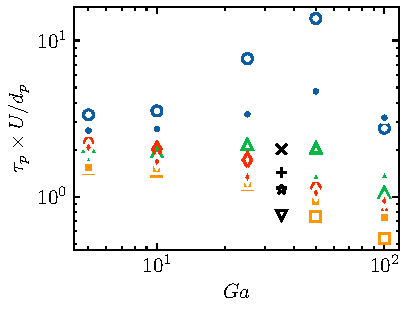
\includegraphics[height = 0.3\textwidth]{image/HOMOGENEOUS_NEW/tau_Ga.pdf}
    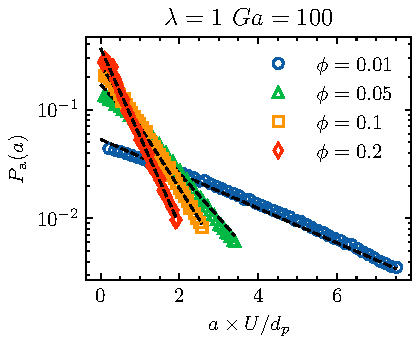
\includegraphics[height = 0.3\textwidth]{image/HOMOGENEOUS_NEW/Dist/Pa_l_1_Ga_100.pdf}
    \caption{
    (left) Mean dimensionless age $\tau_a =  \int_0^\infty aP_a(\textbf{x},t,a)da$ in terms of the \textit{Galileo} number for different volume fraction :   
    ($\pmb\bigcirc$) $\phi = 0.01$; ($\pmb\triangle$) $ \phi = 0.05$; ($\pmb\square$) $\phi = 0.1$ ($\pmb\lozenge$) $\phi = 0.2$.
    The hollow symbols correspond to $\lambda = 1$, the filled symbols to $\lambda = 10$.
    (right) Age distribution function $P_a(\textbf{x},t,a)$ in terms of the dimensionless age, for $\lambda = 1$ and  $Ga = 100$.
    (dashed lines) Theoretical age distribution, see \ref{eq:Pa}. 
    Both the age and the mean age $\tau_a$ are made dimensionless with the drift velocity $U$ and the particle length scale $d_p$.  
    Black symbols represent the DNS results of \citet{zhang2023evolution} for hard sphere suspension with $\phi = 0.0168,0.0565,0.1341,0.2622$, corresponding to the symbols : $\pmb\times, \pmb +, \pmb\star , \pmb\triangledown$, respectively.
    }
    \label{fig:age_picture}
\end{figure}
In \ref{ap:age}  we provided the age distributions but for lower inertial effects, $Ga = 10$. 
It is seen that the age distribution at $\phi = 0.01$ and $Ga = 10$, exhibits a higher density for higher ages and is smaller for small ages, compared to the random distribution.
Therefore, at low \textit{Galileo} and low $\phi$ the \textit{random destruction assumption} doesn't seem to remain valid anymore. 
The \textit{random destruction assumption} must hold true for flows with high particle velocity fluctuation compared to the mean slip velocity, which induces randomness in particle interactions \citep{zhang2023evolution}. 
It is clear that for $\phi \rightarrow 0$, the particle phase fluctuation also tends to $0$, making this condition false. 
Apart from these two cases, it is reasonable to say that \ref{eq:Pa} is well representative of the age distribution function.

In \ref{fig:age_picture} (left) we displayed the dimensionless mean age for all our numerical experiment. 
Regarding the global trend of $\tau_p$, we can say that for almost all of our DNS, the time of interaction is higher for $\lambda = 1$ (hollow symbols) than for $\lambda = 10$ (filled symbols) at same $Ga$ and $\phi$.
Additionally,  $\tau_p$ seem to be well scaled by $U/d_p$ for $\phi  \leq 0.05$ as its values range between $2$ and $0.5$, which is reasonably close to $1$. 
However, $\tau_p$ is clearly superior for $\phi = 0.01$, and reaches a peak for $\phi=0.01$, $Ga=50$, $\lambda=1$.
This, may be correlated with the values of $A_{xx}$ on \ref{fig:A} which also reach a maximum for these parameters. 
Indeed, since $A_{xx}$ is rather high for these simulations, we know that particles are, on average, in a side-by-side configuration, which seems to be a stable configuration since $\tau_p$ is large too.
For $\lambda = 10$ we observe a smaller $\tau_p$ and a smaller $A_{xx}$ at $\phi = 0.01$ and $Ga = 50$, indicating that, on average, the interaction are not as long, while the microstructure is more isotropic. 
The dilute suspension of hard spheres, represented by a $\pmb\times$ symbol, seems to possess even lower $\tau_p$. 
This suggests that solid particles do not necessarily reach a stable equilibrium configuration in the dilute regime, unlike the bubble-like particles ($\lambda = 1$). 
This observation might be explained by the generation of more vorticity in the wake of viscous and solid particles, which makes the interactions less stable at these $Ga$ and $\phi$ values.
These pair interactions mechanisms have been investigated by \citet{yin2008lattice} when studying spherical bubbles and solid particles suspensions.
They reach the conclusion that the weaker wake generated by bubbles tends to make them spend more time in close horizontal orientations, in opposition to solid spherical particles. 
This finding strongly support the previous hypothesis. 
In summary, the mean age of interaction seem to be a good way to measure the particles pairs stability, since it provide a way to measure their interaction time. 
This time is shorter for increasing $\phi$, $\lambda$ and $Ga$, if $\phi \neq 0.01$ in which case it is non-monotonic with $Ga$. 

As mentioned above, $\tau_p(\textbf{x},t)$ is the relaxation time of $\textbf{R}(\textbf{x},t)$. 
Consequently, the microstructure relaxation of dilute suspensions is larger, especially at $Ga = 50$, and may need a consequent amount of time to reach a steady state regime. 
This implies that the terms on the left-hands side of \ref{eq:dt_R} may not be neglected and that direct closure for the microstructure in terms of $\phi$, $Ga$ and $\lambda$ may not be achievable at these large $\tau_p$. 
In turns, this relaxation time will be reflected on the drift velocity between both phases, which is microstructure dependent. 
\begin{figure}
    \centering
    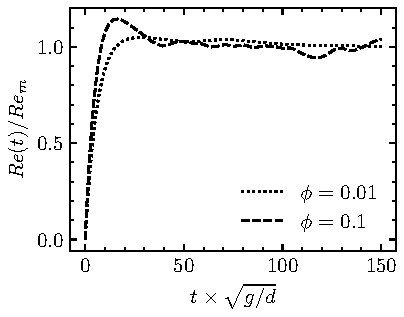
\includegraphics[height=0.325\textwidth]{image/HOMOGENEOUS_NEW/CA/Relax2.pdf}
    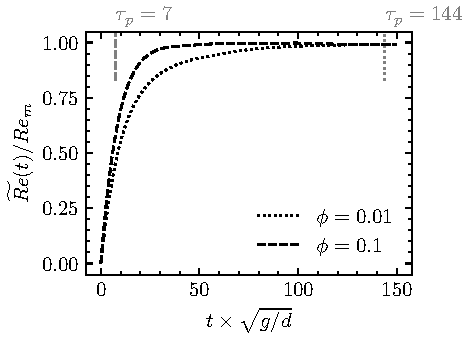
\includegraphics[height=0.35\textwidth]{image/HOMOGENEOUS_NEW/CA/Relax.pdf}
    \caption{
        (left) Average of the Reynolds number based on the instantaneous volume averaged drift velocity, $Re(t) = \rho_fU d /\mu_f$, with $U(t) = |\textbf{u}_p - \textbf{u}_f|$, divided by the mean Reynolds number $Re_m$ in terms of the dimensionless time. 
        (right) Running average of the Reynolds number $\widetilde{Re}(t)$ divided by the mean Reynolds number.
        For $\lambda = 1$ and $Ga = 50$ and two volumes fraction. 
        $\textbf{u}_p$ and $\textbf{u}_f$ are the particle and fluid phase volume averaged velocity at time $t$.
        The verticals gray lines indicate the values of $\tau_p$ all cases. 
        }
        \label{fig:relax}
\end{figure}
Indeed, in \ref{fig:relax} (right) we display the running average of the Reynolds number, based on the drift velocity, divided by the mean Reynolds number of the simulation for two values of $\phi = 0.01,0.1$ at $Ga = 50$ and $\lambda =1$. 
% It is seen that time, at which the simulation reaches a steady state regime is correlated with $\tau_p$. 
In this case we assume that two timescales are involved to bring the drift velocity to its statistically steady state regime. 
The first one is the particles' timescale, which is the time taken for a single particle to reach its own terminal velocity. 
The second timescale is the time taken for the microstructure to go from random, to its steady state microstructure. 
As a matter of fact, on \ref{fig:relax} we see that in the dilute regime ($\phi=0.01$) the rising velocity reaches its averaged value, at a time roughly equal to $100\sqrt{g/d}$ which is of the same order of magnitude than $\tau_p = 144\sqrt{g/d}$. 
On the contrary, when $\phi =0.1$ the averaged Reynolds number is indeed reached earlier ($t = 30\sqrt{g/d}$), despite the higher velocity fluctuations present in this case, see \ref{fig:relax} (left). 
The particle timescale is the same for both cases displayed \ref{fig:relax}, since only the volume fraction changes.
Additionally, the Statistical samples are supposed to be equivalent at same time since each  case posses the same number of droplets per domain. 
Thus, the changes in relaxation time is solely due to the microstructure relaxation timescale. 
Therefore, in support of the theory, $\tau_p$ seems capable of predicting the relaxation time of the microstructure.


The rising velocity of particles is directly correlated to the interphase drag force in sedimentation problems \citep{jackson1997locally}. 
Therefore, in the objective of finding closure terms for the averaged models, one must perform DNS for a time longer than $\tau_p$ plus the particle timescale, to allow the microstructure to relax adequately.
Then by performing an ensemble average procedure, one is able to build drag force models. 
Once established, these models will remain valid only under the condition where the timescale of the macroscopic flow significantly exceeds $\tau_p(\textbf{x},t)$ plus the particle timescale.
Indeed, these models have been built for relaxed microstructure and can be utilized only in this context.
Consequently, $\tau_p$ among other factors such as the particle relaxation time, provides a threshold value for the timescale not achievable in Euler-Euler models. 

\subsubsection*{Particle pairs approach velocity}

\tb{je ne suis plus tellement sur de la pertinience de cette section}

In the next section we will be interested in the velocity fields $\textbf{w}_p^\text{nst}$ since it appear in the source term $\textbf{W}(\textbf{x},t)$, which is at the origin of the modifications of the microstructure, see \ref{eq:dt_R}. 
To give a simpler representation of $\textbf{w}_p^\text{nst}$, we first study the normal approach velocity averaged on all $\textbf{r}$, that is,  
\begin{equation*}
    w_{pn}^aP_a(\textbf{x},t,a)
    = \frac{1}{n_p(\textbf{x},t)}
    \int_{\mathbb{R}^3}
    \frac{\textbf{r}}{r} \cdot \textbf{w}^\text{nst}_p
    P_\text{nst}(\textbf{x},\textbf{r},t,a) d\textbf{r}.
\end{equation*}
In this way, $w^\text{a}_{pn}(\textbf{x},t,a)$ is the average relative normal approach velocity between the nearest pair of particles at age $a$. 
The superscript $^a$ indicate that $w_{pn}^a$ is conditioned only on the age $a$. 
It represents the average approach velocity from one particle to its nearest neighbor, measured from the time when the particles became nearest neighbors, $a=0$.
A scheme of what $\frac{\textbf{r}}{r} \cdot \textbf{w}^\text{nst}_p$ is,  is given \ref{fig:normal_vel_picture} (right). 
\begin{figure}[h!]
    \centering
    % 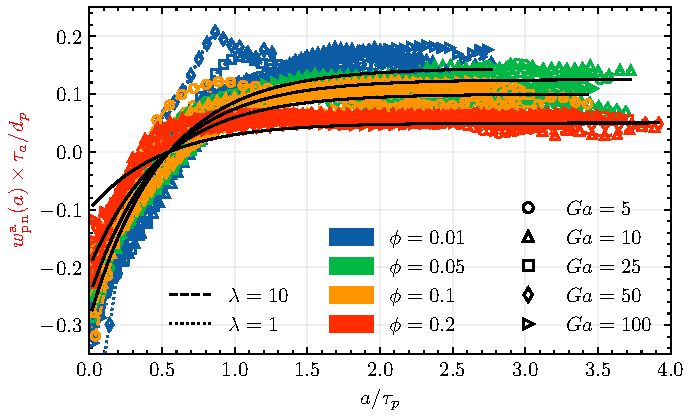
\includegraphics[height = 0.4\textwidth]{image/HOMOGENEOUS_NEW/Age_cond/uR_rel.pdf}
    % \includegraphics[height = 0.3\textwidth]{image/HOMOGENEOUS_NEW/Age_cond/r_l_10_PHI_10.pdf}
    \begin{tikzpicture}[ scale = 0.6]
        \node (img) at (-0.7\textwidth,0){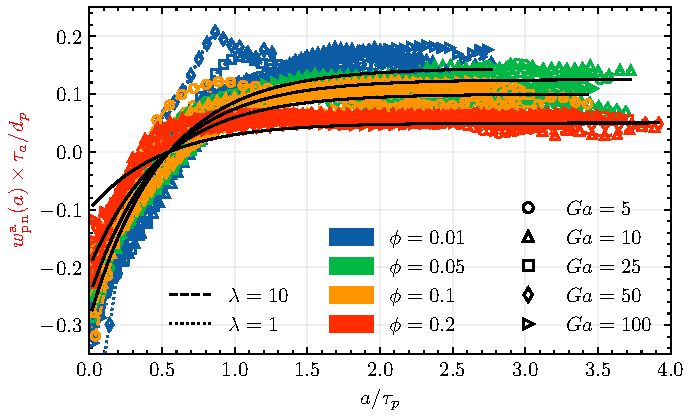
\includegraphics[height = 0.4\textwidth]{image/HOMOGENEOUS_NEW/Age_cond/uR_rel.pdf}};
        \filldraw[ gray!50!white](0,0) circle (0.5);
        \filldraw[ gray!50!white](1,3)circle (0.5);
        % \draw[fill=gray,opacity=0.2](5,-0.2)circle (0.5);
        % \draw[fill=gray,opacity=0.2](-3,2)circle (0.5);
        % \draw[fill=gray,opacity=0.2](-5,0.2)circle (0.5);
        \draw(0,0)node[right]{$\textbf{x}_i$};
        \draw[dashed](0,0)--(1,3)node[right]{$\textbf{x}_j$};
        % \draw[very thick,<-,blue](-1,0)--++(0,1)node[right]{$\bm{b}$};
        \draw[very thick,->](1,3)--++(0.9,-1.8)node[above right]{$\textbf{w}^\text{nst}(a)$};
        \draw[very thick,->,red](1,3)--++(-0.5,-1.5)node[left]{$w_{ij,n}(a)$};
        \draw[dashed](1,3)++(0.9,-1.8) -- (1,3)++(-0.5,-1.5);
        \node (ii) at (1,-1){$\textbf{w}_{ij} = \textbf{u}_j - \textbf{u}_i$};
        \node (ii) at (1,-1.6){$w_{ij,n} = \textbf{w}_{ij}\cdot \textbf{r}/|\textbf{r}|$};
        % \draw[very thick,->](0,0)--++(1,0)node[below right]{$\bm{e_x}$};
        % \draw[very thick,->](0,0)--++(0,1)node[left]{$\bm{e_y}$};
        % \draw(3,1)++(199:1)node[above left]{$\beta$} arc(199:159:1);
        % \draw(0,0)++(0:1)node[above right]{$\theta$} arc(0:20:1);
    \end{tikzpicture} 
    \caption{(left) Relative normal approach velocity between two nearest neighbors, averaged conditionally on the age of interaction.  
    The age $a$, as well as the velocity are made dimensionless  with the mean age $\tau_a$ and the length scale $d_p = n_p^{-1/3}$. 
    % The symbols represent the different \textit{Galileo} numbers, the colors the different 
    % ($\pmb\bigcirc$) $Ga=10$; ($\pmb\triangle$) $ Ga = 25$; ($\pmb\square$) $Ga = 50$ ($\pmb\lozenge$) $Ga =100$.
    % The colors represent the different volume fractions, (blue) $\phi =0.01$, (green) $\phi = 0.05$ (organ) $\phi=0.1$ (red) $\phi = 0.2$. 
    % The white symbols correspond to $\lambda = 1$, and black symbols to $\lambda = 10$. 
    (right)
    Scheme of two nearest neighbors with their position $\textbf{x}_i$ and $\textbf{x}_j$, velocities $\textbf{u}_{i}$ and $\textbf{u}_j$, relative velocity $\textbf{w}_{ij}$ and normal relative velocity $w^{ij,n}$. 
    }
    \label{fig:normal_vel_picture}
\end{figure}
The approach velocity $w_{pn}^a(\textbf{x},t,a)$ for all the DNS carried in this work is displayed \ref{fig:normal_vel_picture} (left). 
The x-axis is made dimensionless with the averaged time of interaction, $\tau_p$, and the y-axis is scaled with the velocity scale $d_p /\tau_p$. 
At  early age we observe that $w_{pn}^a<0$.
Then it eventually reaches zero for  $a \approx 0.5\tau_p$.
After this time $w_{pn}^a>0$ and remains constant with respect to $a$. 
Hence, on average, particles approach each other at early ages ($w_{pn}^a<0$), and then they move apart for $a > \tau_p$ with a constant average velocity.

Two important features are identified from \ref{fig:normal_vel_picture} (left).
First, all curves are roughly similar, even if we can see slight differences in magnitude for the different $\phi$. 
Thus, regardless of the flow parameters, $w_{pn}^a(\textbf{x},t,a)$ scale roughly as $d_p /\tau_p$. 
Second,  $w_{pn}^a(\textbf{x},t,a)$ seems to relax for age, $a > \tau_p$, to reaches a constant value. 
% Consequently, it seems that $\tau_p$ is also the relaxation time for the particles' relative normal approach velocity. 
Consequently, we demonstrated that $\tau_p$ and $d_p$ were the correct time and length scale which govern the inter particle scale kinematics   and that $\tau_p$ is also the relaxation time of $w_{pn}^a(\textbf{x},t,a)$. 
% It is clear that all nearest averaged property will be also subject to a relaxation time $\tau_p$, this in fact comes from the structure of the nearest particle averaged probability transport equation (\ref{eq:dt_Pnst}) which makes appear this relaxation time. 
In general, we believe that $w_{pn}^a(\textbf{x},t,a)$ might be useful for the future studies aiming to construct models based on the relative velocity between particles \citep{rao2008introduction}. 

